\documentclass[11pt,a4paper]{article}
\usepackage[margin=1.9cm,top=1.8cm,bottom=1.9cm]{geometry}
\usepackage[T1]{fontenc}\usepackage[utf8]{inputenc}\usepackage[brazil]{babel}
\usepackage{lmodern,microtype,amsmath,booktabs,array,graphicx,float,caption,xcolor,enumitem,fancyhdr,hyperref}
\definecolor{ink}{HTML}{163447}\hypersetup{colorlinks=true,urlcolor=ink,linkcolor=ink}
\setlength{\parindent}{0pt}\setlength{\parskip}{6pt}\setlength{\headheight}{15pt}
\setlength{\tabcolsep}{5pt}\renewcommand{\arraystretch}{1.10}
\setlength{\intextsep}{6pt}\setlength{\textfloatsep}{8pt}\setlist{nosep}
\captionsetup{font=small,labelfont=bf,skip=4pt}
\pagestyle{fancy}\fancyhf{}\fancyhead[L]{\small Termos de troca e risco cambial}\fancyhead[R]{\small Complemento ao segundo estudo}\fancyfoot[C]{\thepage}
\renewcommand{\headrulewidth}{.3pt}\setlength{\emergencystretch}{2em}
\begin{document}
\section*{Termos de troca, câmbio real e risco do carrego}
\begin{center}\large Complemento ao segundo relatório\\[5pt]\normalsize Testes de previsão, alertas e saída de posições\\11 de setembro de 2026\end{center}
\vspace{8pt}
\textbf{Pergunta.} Se as condições comerciais de um país mudam, a referência de longo prazo do câmbio real pode mudar também. Uma moeda aparentemente barata pode deixar de convergir ao patamar antigo. Conseguimos antecipar isso e evitar carregar uma posição mais arriscada?

\textbf{Resposta empírica.} Há sinais úteis para investigar, mas não encontramos uma cadeia robusta que permita concluir ``previ mudança estrutural, portanto devo sair''. A previsão da composição comercial perde para a persistência. Acrescentar preços comerciais melhora modestamente alguns modelos reais longos, mas eles continuam piores que nenhuma mudança. Na carteira, mudanças \emph{já observadas} na composição e saídas por probabilidade de perda foram mais interessantes que o simples alerta de mudança prevista.
\small\begin{center}\begin{tabular}{ll}\toprule Teste & Resultado principal\\\midrule 
Prever composição comercial & RMSE 1,20 vez a persistência\\
Prever termos agregados anuais & RMSE 0,86; somente seis anos avaliados\\
Prever perda do carrego & Brier relativo 0,93; sem significância após Holm\\
Filtro de composição observada & Melhora descritiva de retorno/risco\\
Saída de coortes por risco & Menor queda; ganho médio incerto\\\bottomrule\end{tabular}\end{center}\normalsize

\textbf{Escopo.} Reaplicamos os testes relevantes do segundo estudo: quando carregar, tamanho, saídas, câmbio consumir juros, perda no caminho e caudas. O terceiro estudo fornece os preços e a construção comercial inicial. Os três relatórios anteriores foram preservados.

\textbf{Como ler.} Resultados são fora da amostra de estimação a cada data, mas exploratórios dentro de uma história já examinada. Uma queda menor com menos exposição não prova capacidade de prever risco. Por isso incluímos controles de exposição e de volatilidade, custos e resultados desfavoráveis.

\clearpage
\section*{1. O mecanismo econômico que estamos testando}

Definimos $s$ como log de moeda local por dólar e $q=s+p_{US}-p_i$. Aumento de $q$ significa depreciação real da moeda local. O retorno cambial de uma posição comprada nessa moeda tem o sinal oposto à variação de $s$.

Uma melhora dos termos de troca pode alterar renda externa, demanda e preços relativos; uma deterioração pode alterar o caminho inverso. \textbf{O sinal e a persistência são hipóteses a testar}, sem impor que todo choque produza apreciação/depreciação permanente.

Distinguimos três objetos:
\begin{enumerate}
\item \textbf{Termos de troca agregados}: preço das exportações relativamente ao preço das importações, incluindo bens além das commodities.
\item \textbf{Exposição aos preços de commodities}: quanto movimentos em energia, alimentos, matérias-primas e metais afetam a cesta comercial aproximada do país.
\item \textbf{Composição comercial}: mudanças nas participações e na exposição líquida desses grupos. Usamos valores de comércio; suas mudanças também refletem preços. Não identificam, sozinhas, transformação produtiva ou quebra estrutural.
\end{enumerate}

O teste tem três etapas distintas: prever a informação comercial; acrescentá-la à previsão real/nominal ou à probabilidade de perda; usar somente a previsão disponível para decidir a posição. Sucesso numa etapa não garante sucesso na seguinte.

\textbf{Exemplo.} Se o país passa a exportar relativamente mais energia, sua sensibilidade ao petróleo pode mudar. Mas sair de uma posição comprada apenas por detectar essa mudança ignora se o petróleo vai subir ou cair, se o câmbio já incorporou a notícia e se o diferencial de juros compensa o risco. Os testes de sinal e de risco tentam separar essas possibilidades.

\textbf{Limite do exercício.} Chamamos de ``referência real persistente'' a média realizada de 12 meses ao final do horizonte. Ela é mensurável; não equivale a estimar um câmbio de equilíbrio estrutural permanente.

\clearpage
\section*{2. Dados e relógio da informação}

Mantemos BRL, EUR, JPY, GBP, CAD e SEK, com conta em USD. Para o comércio do euro, Alemanha é uma proxy imperfeita; há sensibilidade sem EUR. Câmbio, CPI e juros vêm dos estudos anteriores. Preços mensais são as cestas da Pink Sheet do Banco Mundial; não são retornos de futuros.

Baixamos 11 séries anuais WDI: valores totais exportados/importados, oito participações setoriais e o índice agregado UNCTAD de termos de troca. Fluxos/participações cobrem 1994--2024 de forma suficiente para os pesos usados. A edição obtida do índice agregado tem 2005--2024 para as seis economias.

Os pesos anuais líquidos são
\[
w_{i,k,y}=\frac{X_{i,y}a^X_{i,k,y}-M_{i,y}a^M_{i,k,y}}{X_{i,y}+M_{i,y}}.
\]
No ano $Y$, admitimos apenas dados até $Y-2$ e usamos média de três anos. A sensibilidade usa $Y-3$. É uma convenção conservadora, não a data de publicação efetivamente reconstruída de cada observação.

Com preços setoriais $b_{k,t}$ em log, encadeamos
\[
Z_{i,t}=Z_{i,t-1}+\sum_k \bar w_{i,k,Y(t)-2}\,(b_{k,t-1}-b_{k,t-2}).
\]
O índice não salta apenas porque os pesos mudaram ou porque uma commodity foi cotada em outra unidade. A versão fixa usa 1994--1996. $Z$ é uma proxy de exposição comercial a preços, não o índice oficial de termos de troca agregados.

CPI entra com dois meses de atraso, com preenchimento de no máximo um mês passado, conforme o estudo original. Preços mensais entram com um mês. Nenhuma interpolação usa anos futuros. Os arquivos brutos e hashes estão no pacote.

\textbf{Vintages.} As séries foram baixadas na edição atual. Atrasar sua entrada impede uso direto do futuro, mas não desfaz revisões históricas. Participações em valor e a proxy alemã limitam a interpretação econômica.

\clearpage
\section*{3. Previsão real e comparação justa}

Dois alvos são previstos diretamente para $h=12,36,60$ meses:
\[
Y^q_{i,t,h}=q_{i,t+h}-q_{i,t-2},\qquad
Y^{\bar q}_{i,t,h}=\frac1{12}\sum_{j=0}^{11}q_{i,t+h-j}-q_{i,t-2}.
\]
A base é o último câmbio real inteiramente conhecido, $t-2$. Assim, o endpoint está $h$ meses depois da origem, e $h+2$ depois da base. Prever nenhuma mudança significa zero para esses alvos.

O modelo base contém desvio histórico do câmbio real e sua mudança em 12 meses, interceptos de país e ridge fixa 10, padronizada apenas no treino. Acrescentamos separadamente:
\begin{itemize}
\item nível/desvio e momentum do índice comercial de pesos fixos;
\item os mesmos termos com pesos variáveis;
\item nível e mudança dos termos agregados anuais;
\item magnitude da mudança de composição observada, magnitude prevista e cenário de reprecificação dessa composição;
\item conjunto de informações variáveis, anuais e de composição.
\end{itemize}

O cenário de reprecificação multiplica a mudança prevista dos pesos pelos preços relativos às suas médias passadas de 36 meses. Sua unidade não depende do nível arbitrário dos preços; não é uma estimativa causal de equilíbrio.

\textbf{Mesma história para o benchmark.} Para cada modelo aumentado, reestimamos a base exatamente nas mesmas linhas de treino. Sem isso, descartar anos antigos por falta de dados comerciais poderia parecer ganho informacional. O calendário de previsão e a amostra de avaliação também são pareados por comparação.

Treino em expansão, mínimo de 60 datas por moeda. O alvo real só entra depois de realizado e publicado, com buffer adicional de um mês. Modelos com informações anuais/previsões recursivas começam mais tarde. As tabelas mostram esse custo de disponibilidade.

\clearpage
\section*{4. Os preços comerciais preveem o câmbio real?}
\small\begin{center}\begin{tabular}{lrrrr}\toprule h & Informação adicional & Origens & RMSE/base & RMSE/zero\\\midrule 
12 & Preços / pesos fixos & 152 & 1,010 & 1,191\\
12 & Preços / pesos variáveis & 152 & 1,020 & 1,203\\
36 & Preços / pesos fixos & 128 & 0,976 & 1,755\\
36 & Preços / pesos variáveis & 128 & 0,978 & 1,758\\
60 & Preços / pesos fixos & 104 & 0,958 & 2,104\\
60 & Preços / pesos variáveis & 104 & 0,948 & 2,083\\\bottomrule\end{tabular}\end{center}\normalsize
\begin{figure}[H]\centering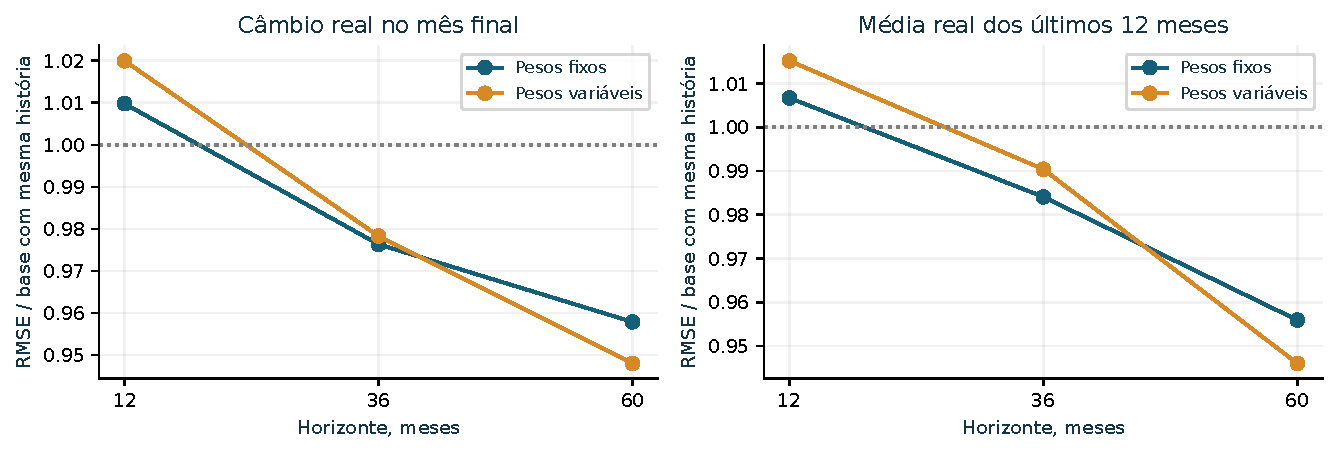
\includegraphics[width=.98\linewidth]{figures/real_gain.pdf}\caption{Pequenas melhoras sobre a regressão de reversão real em horizontes longos. As linhas não mostram vitória sobre nenhuma mudança.}\end{figure}
Em 60 meses, pesos variáveis reduzem o erro em cerca de 5\% frente à base pareada. Porém, o RMSE continua superior a duas vezes o de prever nenhuma mudança. A inclusão melhora um modelo que está falhando nesse benchmark mais exigente.

No horizonte de 12 meses, os preços comerciais pioram a base. Trocar pesos fixos por variáveis não produz melhora uniforme. Esses resultados não sustentam que a exposição comercial, sozinha, resolva a previsão do câmbio real de longo prazo.

\clearpage
\section*{5. A referência real persistente muda de forma previsível?}
\small\begin{center}\begin{tabular}{lrrrr}\toprule h & Informação & Origens & RMSE/base & RMSE/zero\\\midrule 
36 & Preços / pesos variáveis & 128 & 0,990 & 1,726\\
36 & Termos agregados anuais & 90 & 1,198 & 1,804\\
36 & Composição e previsão & 54 & 1,109 & 0,974\\
36 & Todas as informações & 54 & 1,003 & 0,881\\
60 & Preços / pesos variáveis & 104 & 0,946 & 2,141\\
60 & Termos agregados anuais & 42 & 1,085 & 1,386\\
60 & Composição e previsão & 6 & 1,422 & 1,126\\
60 & Todas as informações & 6 & 1,548 & 1,226\\\bottomrule\end{tabular}\end{center}\normalsize
\begin{figure}[H]\centering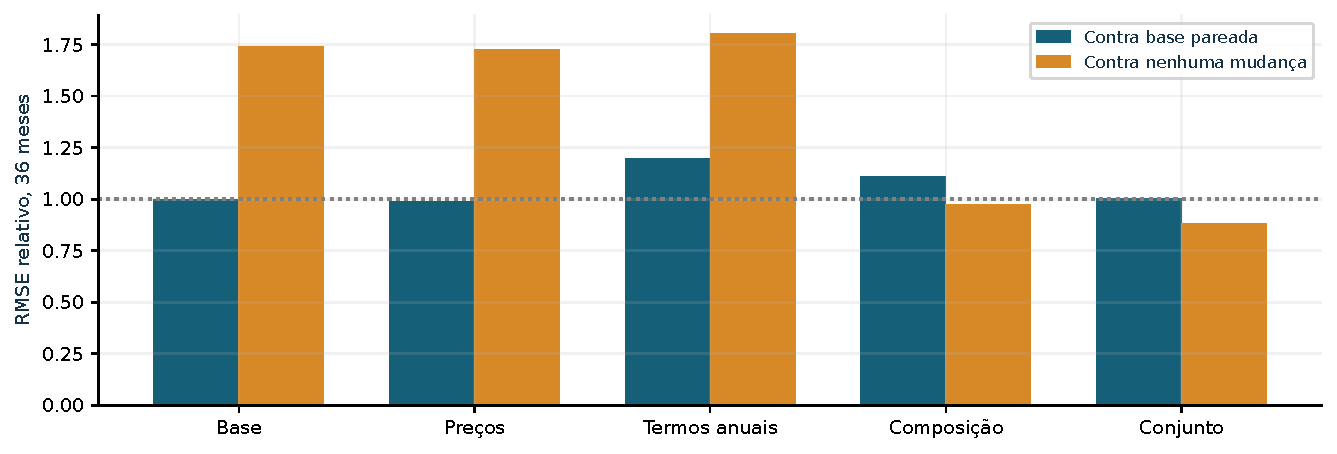
\includegraphics[width=.98\linewidth]{figures/persistent_benchmarks.pdf}\caption{Modelos de 36 meses usam 128, 90 ou 54 origens conforme disponibilidade. Cada razão contra a base usa a mesma história do modelo correspondente.}\end{figure}
A previsão conjunta da média real futura em 36 meses fica abaixo de nenhuma mudança na janela curta em que pode ser avaliada. Mas quase não melhora sua base reestimada na mesma história: a razão é aproximadamente 1,003. Logo, a aparente vitória não pode ser atribuída à informação comercial acrescentada.

Em 60 meses, o bloco de composição e o conjunto têm somente seis origens comuns avaliáveis, todas em 2021. Não há suporte para inferência. A disponibilidade tardia é um resultado de viabilidade relevante, e não deve ser escondida combinando moedas como se fossem décadas independentes.

\clearpage
\section*{6. E o câmbio nominal previsto pelo EJR?}
\small\begin{center}\begin{tabular}{lrrrr}\toprule h & Modelo & Origens & RMSE/EJR & RMSE/zero\\\midrule 
12 & EJR & 152 & 1,000 & 1,051\\
12 & Fixed & 152 & 1,055 & 1,109\\
12 & Dynamic & 152 & 1,061 & 1,116\\
36 & EJR & 128 & 1,000 & 1,259\\
36 & Fixed & 128 & 1,120 & 1,410\\
36 & Dynamic & 128 & 1,126 & 1,417\\
60 & EJR & 104 & 1,000 & 1,357\\
60 & Fixed & 104 & 1,001 & 1,358\\
60 & Dynamic & 104 & 0,985 & 1,337\\\bottomrule\end{tabular}\end{center}\normalsize

Aqui preservamos o EJR original como referência: inclinação agrupada, sem intercepto, desvios reais centralizados somente com informação disponível. As extensões acrescentam fator comum dos preços e a proxy comercial fixa ou variável, sob a mesma restrição de regressão.

Os resultados não mostram uma melhora generalizada. A versão variável apresenta ganho pequeno em cinco anos frente ao EJR, mas permanece pior que nenhuma mudança. Em 12 e 36 meses, as extensões pioram a previsão.

\textbf{Relação com o terceiro relatório.} O terceiro destacou um componente comercial específico em outra construção e janela. Este complemento começa a avaliação em 2013, usa índices comerciais encadeados, inclui pesos anuais variáveis e tem foco em risco. Não se deve transpor o ganho do terceiro relatório para estas carteiras como se fosse uma propriedade universal do sinal.

\textbf{Interpretação.} Um país mudar sua exposição comercial não basta para prever a direção do nominal. Política monetária, inflação relativa, preços já incorporados e outros fatores podem absorver o ajuste. A análise é preditiva e não identifica causalidade entre comércio e câmbio.

\clearpage
\section*{7. Conseguimos antecipar as próprias condições comerciais?}
\small\begin{center}\begin{tabular}{lrr}\toprule Alvo e regra & Anos & RMSE/persistência\\\midrule 
Composição: ridge & 12 & 1,199\\
Composição: extrapolar tendência & 12 & 1,421\\
Termos agregados: ridge & 6 & 0,856\\
Termos agregados: tendência & 6 & 2,682\\\bottomrule\end{tabular}\end{center}\normalsize

\textbf{Composição.} Em cada ano $Y$, prevemos os pesos suavizados do ano $Y+1$ a partir dos últimos conhecidos, $Y-2$. O horizonte entre dados é de três anos. Entram níveis e mudanças passadas dos pesos; o treinamento usa anos completos, cada ano uma única vez por país. Ridge fixa e pelo menos oito anos de treino. Persistência é mudança prevista zero.

O erro da previsão de composição é cerca de 20\% maior que a persistência; extrapolar a tendência é ainda pior. Algumas economias têm resultados anuais de 2025 enquanto outras não; as métricas usam apenas células realizadas e mostram a contagem nos CSVs. Não há evidência agregada de que antecipamos bem a transformação da cesta.

\textbf{Termos agregados.} Um exercício anual adicional usa nível e última variação do índice, prevendo a mudança entre $Y-2$ e $Y+1$. A ridge supera a persistência na amostra disponível, mas só há seis origens anuais, 2018--2023, com alvos sobrepostos. Este resultado é um piloto e não foi usado como filtro de carteira validado.

\textbf{Exposição mensal aos preços.} Prevemos a mudança de $Z$ em 12 meses com nível e momentum históricos. A razão de RMSE contra zero é 1,071. O ganho de timing não pode ser presumido: o próprio primeiro estágio é fraco.

As previsões de composição e de $Z$ são geradas recursivamente antes de entrarem no modelo de risco. Nenhuma previsão ajustada com a amostra completa é usada como sinal histórico.

\clearpage
\section*{8. Repetição dos testes de risco do segundo relatório}
\small\begin{center}\begin{tabular}{lrrrr}\toprule Alvo & Preços var. & Termos anuais & Composição & Conjunto\\\midrule 
Juros consumidos, 12m & 1,034 & 1,011 & 0,962 & 1,005\\
Perda adversa, 12m & 1,111 & 1,010 & 1,074 & 1,224\\
Perda adversa, 36m & 0,983 & 1,137 & 1,154 & 1,214\\
Perda adversa, 60m & 1,013 & 1,040 & 1,147 & 1,270\\
Tempo negativo, 12m & 1,046 & 1,015 & 0,980 & 1,044\\
Tempo negativo, 36m & 0,991 & 1,028 & 0,998 & 1,002\\
Tempo negativo, 60m & 1,040 & 1,002 & 1,091 & 1,094\\
Cauda agregada, 1m & 1,025 & 1,014 & 1,000 & 1,050\\
Cauda agregada, 3m & 1,017 & 1,036 & 1,014 & 1,128\\\bottomrule\end{tabular}\end{center}\normalsize

Cada célula é RMSE do modelo aumentado dividido pelo da base reestimada na mesma história. Para alvos binários, o quadrado dessa razão é a razão de Brier. A base contém diferencial de juros em valor absoluto, volatilidade, momentum e previsão EJR, orientados pelo sinal da posição. Interceptos de país não são penalizados; a ridge tem penalidade 10. Reaplicamos a família de testes, sem alterar os números antigos.

\textbf{Juros consumidos.} O bloco de composição reduz o Brier em aproximadamente 7,4\%, com AUC 0,600 em 126 origens mensais. O p-valor ajustado por Holm é 0,650. É um candidato exploratório, não uma melhora estatisticamente estabelecida.

\textbf{Perda no caminho.} O alvo é o pior retorno log acumulado, abaixo da entrada, mantendo a direção inicial da moeda e somando o diferencial de juros realizado. Não é o máximo drawdown desde um pico intermediário, nem inclui custos de carteira. O tempo negativo mede a fração do caminho abaixo da entrada.

\textbf{Caudas.} Repetimos perdas agregadas de excesso de retorno inferiores a 2\% em um mês e 4\% em três meses, com a contabilidade líquida da carteira original. As informações comerciais não melhoram essas previsões de forma consistente.

As janelas variam por informação e horizonte: em perdas de 60 meses, há apenas 30--42 origens. O conjunto mais rico frequentemente piora o resultado, mostrando o custo de acrescentar variáveis em uma amostra pequena.

\clearpage
\section*{9. Do sinal à decisão de carregar ou sair}

Os alertas são definidos antes da execução. O corte principal é o percentil 80 da história do próprio sinal em cada moeda, calculado apenas até o mês anterior, com no mínimo 36 observações. Também testamos 70/90 e retirada de metade da exposição.
\footnotesize\begin{center}\begin{tabular}{ll}\toprule Alerta & Informação usada\\\midrule 
Preços observados & Deterioração direcional de Z em 12 meses\\
Preços previstos & Deterioração direcional prevista de Z em 12 meses\\
Composição observada & Soma das mudanças absolutas dos pesos em três anos\\
Composição prevista & Soma das mudanças absolutas previstas dos pesos\\
Revisão real 36/60m & Previsão da média real com preços menos base pareada\\
Depreciação real 60m & Previsão direcional do câmbio real final\\
Aumento do risco & Probabilidade com composição menos base pareada\\\bottomrule\end{tabular}\end{center}\normalsize

Nos sinais direcionais, o alerta é invertido para posições vendidas. Magnitudes de composição são alertas simétricos. Cada par carry tem 25\% comprado e 25\% vendido. Se uma perna aciona o alerta, retiramos o par inteiro, sem redistribuir seu risco aos outros pares.

Sobrepomos cada alerta a carry puro, ao filtro EJR de retorno total acima de 2\% a.a. suavizado em seis meses e ao dimensionamento gradual EJR do segundo estudo. Coortes abrem pequenas posições mensais, expiram em 12 meses e, quando fechadas por alerta, permanecem em caixa até sua expiração. A avaliação começa quando todos os sinais da comparação estão disponíveis.

\textbf{Execução e retorno.} Sinal no fechamento $t$, operação em $t+1$, primeiro retorno em $t+2$. Usamos o mesmo motor do segundo relatório: ativo estrangeiro convertido a USD, funding em USD, remuneração do caixa, spread de empréstimo nas pernas vendidas, giro, entrada e liquidação final. Custos cambiais em pontos-base: BRL 10; EUR/JPY/GBP/CAD 2; SEK 3. Spread anual de empréstimo 50 pontos-base. Há sensibilidade a custos duplicados.

O alerta estatístico acima do percentil é uma regra de ranking histórica. Ele não exige que uma revisão real seja positiva em nível absoluto. Portanto, testa deterioração relativa do sinal, e não um limite universal de risco.

\clearpage
\section*{10. Todos os filtros sobre o carry puro}
\footnotesize\begin{center}\begin{tabular}{lrrrrr}\toprule Filtro & Início & Exp. & Excesso a.a. & Vol. & Maior queda\\\midrule 
Piora de preços observada & 2013-03 & 64,20\% & 1,83\% & 3,29\% & -7,10\%\\
Piora de preços prevista & 2013-03 & 76,85\% & 1,32\% & 3,73\% & -8,67\%\\
Composição observada & 2013-03 & 69,75\% & 2,82\% & 3,53\% & -8,10\%\\
Composição prevista & 2014-03 & 72,33\% & 1,68\% & 3,67\% & -9,04\%\\
Revisão real em 36m & 2013-03 & 66,36\% & 1,09\% & 2,96\% & -9,09\%\\
Revisão real em 60m & 2014-04 & 92,62\% & 2,58\% & 4,21\% & -9,09\%\\
Depreciação real em 60m & 2014-04 & 54,36\% & 1,06\% & 3,04\% & -9,14\%\\
Aumento da probabilidade de perda & 2018-04 & 82,67\% & 2,74\% & 3,60\% & -7,46\%\\\bottomrule\end{tabular}\end{center}\normalsize
\begin{figure}[H]\centering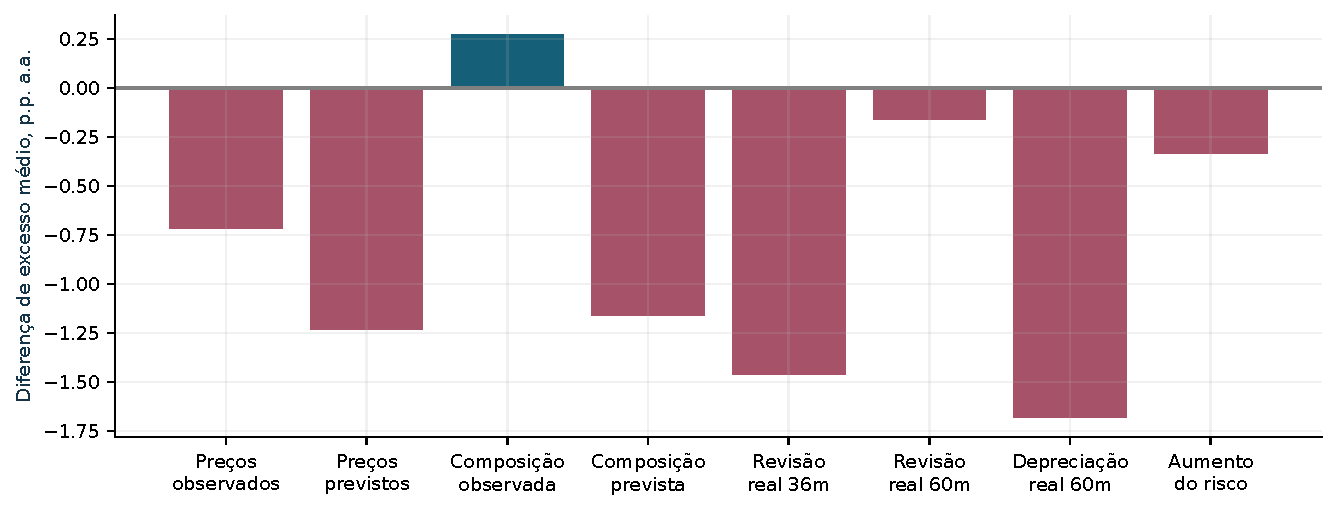
\includegraphics[width=.98\linewidth]{figures/all_filters.pdf}\caption{Cada diferença usa seu carry de referência nas mesmas datas. Os filtros têm inícios distintos por disponibilidade, sem escolher a janela pelo desempenho.}\end{figure}
A maioria dos filtros reduz o retorno médio. O alerta de composição observada é uma exceção nesta amostra. Preços previstos e composição prevista retiram exposição sem compensação clara. A revisão da referência real tampouco produz regra robusta de saída.

Uma estratégia ficar menos volátil após retirar posições é esperado. A tabela seguinte e os controles de exposição verificam se o resultado vai além desse efeito mecânico.

\clearpage
\section*{11. Candidato: composição observada}
\begin{figure}[H]\centering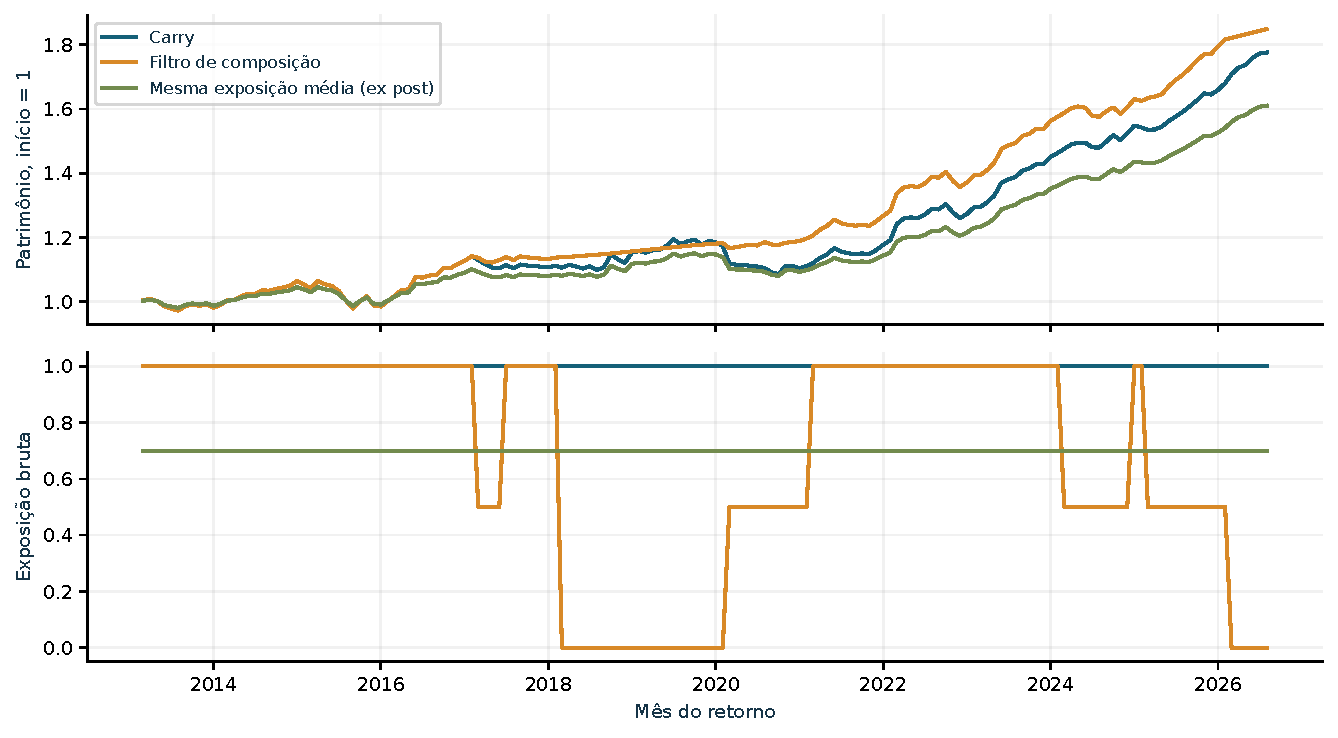
\includegraphics[width=.98\linewidth]{figures/structure_wealth.pdf}\caption{Retornos líquidos e exposição desde março de 2013. O controle de mesma exposição média é calculado ex post e serve apenas como diagnóstico.}\end{figure}\small\begin{center}\begin{tabular}{lrrrrr}\toprule Regra & Exp. & Excesso a.a. & Vol. & Sharpe & Maior queda\\\midrule 
Carry & 100,00\% & 2,55\% & 4,22\% & 0,61 & -9,09\%\\
Composição & 69,75\% & 2,82\% & 3,53\% & 0,81 & -8,10\%\\
Exposição passada & 82,89\% & 2,01\% & 3,62\% & 0,56 & -8,10\%\\
Exposição ex post & 69,75\% & 1,78\% & 2,98\% & 0,61 & -6,13\%\\\bottomrule\end{tabular}\end{center}\normalsize

O filtro reduz a exposição média para cerca de 70\%. O excesso médio sobe de 2,55\% para 2,82\% a.a., e a volatilidade cai de 4,22\% para 3,53\%. Desde 2019, a maior queda cai de 9,09\% para 3,37\%. Sobre o dimensionamento EJR, o excesso sobe de 2,80\% para 3,11\% a.a.

Isso é compatível com evitar certas posições após mudança comercial, mas não prova previsão de quebra. Nos meses de alerta, o carry bruto da regra de saída teve retorno médio menor, sem uma frequência de cauda uniformemente maior. O canal pode ser seleção de retorno, não apenas identificação de risco extremo.

\textbf{Proteção à mesma exposição.} O filtro tem volatilidade e maior queda superiores ao controle de exposição média ex post. Seu atrativo é a relação entre retorno e risco nesta amostra; não é uma dominância de proteção sobre simplesmente carregar menos.

\clearpage
\section*{12. Candidato: sair de coortes quando o risco sobe}
\begin{figure}[H]\centering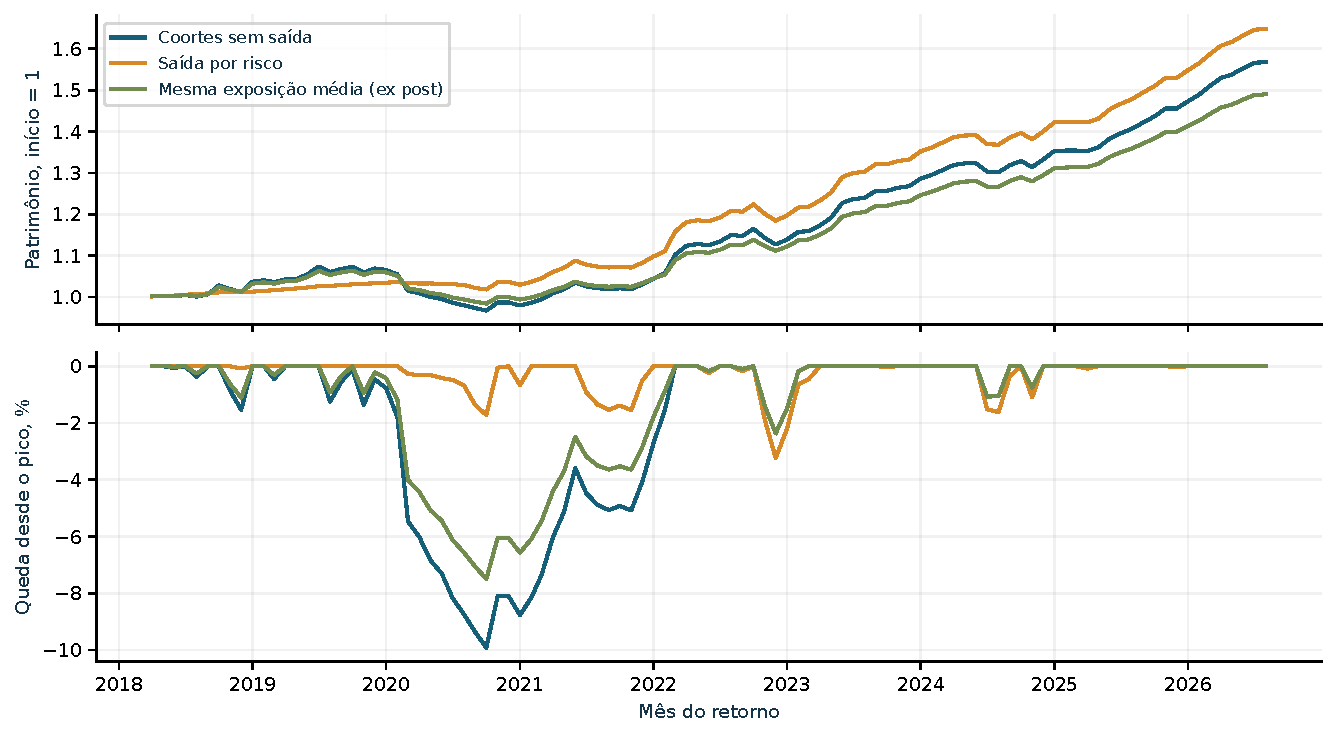
\includegraphics[width=.98\linewidth]{figures/cohort_risk.pdf}\caption{Coortes de 12 meses, abril de 2018 a agosto de 2026. A saída responde ao acréscimo da probabilidade prevista de o câmbio consumir os juros.}\end{figure}\small\begin{center}\begin{tabular}{lrrrrr}\toprule Regra & Exp. & Excesso a.a. & Vol. & Sharpe & Maior queda\\\midrule 
Manter coortes & 94,55\% & 2,78\% & 3,80\% & 0,74 & -9,92\%\\
Sair por risco & 72,94\% & 3,34\% & 3,00\% & 1,12 & -3,23\%\\
Exposição ex post & 72,94\% & 2,14\% & 2,95\% & 0,74 & -7,50\%\\\bottomrule\end{tabular}\end{center}\normalsize

Esta é a versão mais próxima da hipótese do usuário: a informação comercial muda a avaliação de risco e encerra a posição antes do vencimento. O maior drawdown passa de 9,92\% para 3,23\%, e o excesso médio de 2,78\% para 3,34\% a.a. A regra mensal sem coortes é menos convincente: reduz retorno e o ganho de Sharpe é pequeno.

O resultado usa apenas 101 meses e depende do desenho da saída. Cortes e custos adicionais aparecem nas sensibilidades. Redução observada de drawdown não demonstra que o próximo choque será evitado.

Contra a mesma exposição média ex post, a redução de drawdown é 4,26 pontos percentuais, com intervalo condicional de 95\% de $[-0,86;10,38]$ em blocos de 12 meses. A diferença de volatilidade é quase nula. Portanto, a melhora de proteção além da exposição não está estabelecida estatisticamente.

\clearpage
\section*{13. Proteção sobre o filtro EJR de 2\% a.a.}
\begin{figure}[H]\centering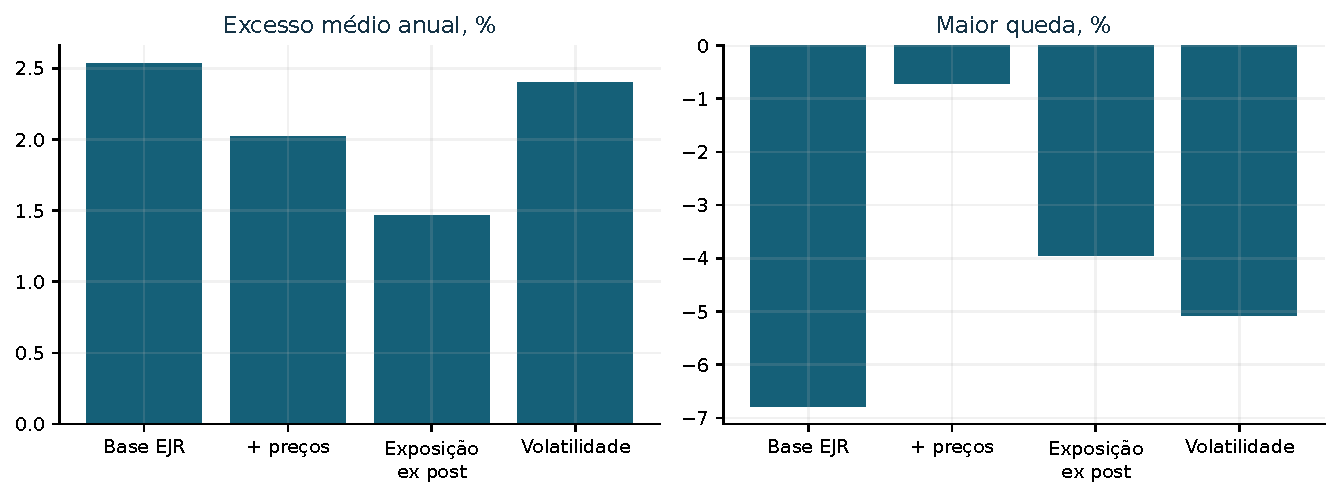
\includegraphics[width=.98\linewidth]{figures/ejr_price.pdf}\caption{Acrescentar deterioração observada dos preços ao filtro EJR reduz risco e também retorno. Todos os controles usam março de 2013 a agosto de 2026.}\end{figure}
O filtro EJR original desta comparação tem excesso médio de 2,53\% a.a. e maior queda de 6,78\%. Acrescentar o alerta de preços observados leva o excesso a 2,02\% e a queda a 0,72\%, com exposição média próxima de 21\%.

Esse resultado parece forte como proteção, mas o controle com exposição reduzida também apresenta risco muito baixo. O controle de exposição calculado somente com o passado é operacional, porém não iguala exatamente a exposição média realizada. O controle ex post iguala a média, mas usa informação futura e não é uma estratégia implementável.

\textbf{Qual escolha este teste informa?} Um investidor disposto a sacrificar retorno para reduzir exposição em condições comerciais adversas pode preferir esse tipo de filtro. O exercício não demonstra que essa troca domina uma redução simples do orçamento de risco.

O objetivo foi separar três perguntas: o sinal melhora previsão? Ele seleciona retornos? Ele protege além do efeito de manter menos risco? Elas têm respostas diferentes. A melhora visual de uma curva de patrimônio não substitui as comparações preditivas e de exposição.

\clearpage
\section*{14. Sensibilidade: o padrão permanece?}
\small\begin{center}\begin{tabular}{lrrrr}\toprule Variação & Obs.: $\Delta$Sharpe & Obs.: $\Delta$ret. & Prev.: $\Delta$Sharpe & Prev.: $\Delta$ret.\\\midrule 
Base & 0,19 & 0,27 & -0,20 & -1,16\\
Ridge1 & 0,19 & 0,27 & -0,08 & -0,76\\
Ridge100 & 0,19 & 0,27 & -0,05 & -0,61\\
Lag3 & 0,14 & 0,23 & 0,30 & 0,07\\
NoBRL & -0,16 & -0,56 & 0,02 & -0,11\\
NoEUR & 0,18 & 0,27 & -0,21 & -1,07\\\bottomrule\end{tabular}\end{center}\normalsize
\begin{figure}[H]\centering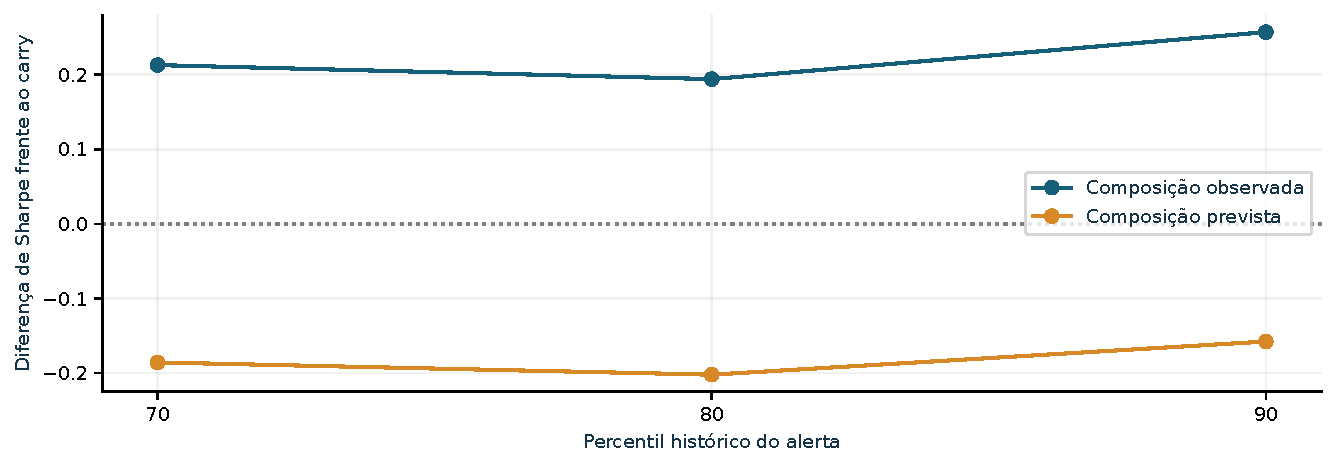
\includegraphics[width=.98\linewidth]{figures/thresholds.pdf}\caption{Diferença de Sharpe para três cortes previamente definidos. Mudanças de corte não são testes independentes.}\end{figure}
$\Delta$ret. está em pontos percentuais anuais contra o carry da mesma variante. Sem BRL/EUR, refazemos o ranking no universo restante; o benchmark muda junto. O atraso de três anos muda o momento do sinal e o horizonte da previsão anual para quatro anos.

\textbf{Fragilidade relevante.} Composição prevista tem resultado fraco na especificação principal, mas melhora bastante ao atrasar mais um ano. Isso merece investigação sobre atualização dos dados e defasagem econômica, não seleção automática da melhor versão. A sensibilidade é incompatível com uma regra já estável.

Os modelos reais também foram reestimados com ridge 1/100, janela 120 meses e exclusão de moedas. Os resultados completos estão nos CSVs. Para as políticas, ``Window120'' mantém o alerta anual original; a janela móvel pertence à regressão real, não altera artificialmente o sinal anual.

\clearpage
\section*{15. Variações da saída e incerteza dos ganhos}
\small\begin{center}\begin{tabular}{lrrrrr}\toprule Percentil & Custo $\times$ & Exp. & Excesso a.a. & Sharpe & Maior queda\\\midrule 
70 & 1 & 64,40\% & 3,04\% & 1,06 & -3,23\%\\
70 & 2 & 64,40\% & 3,01\% & 1,06 & -3,24\%\\
80 & 1 & 72,94\% & 3,34\% & 1,12 & -3,23\%\\
80 & 2 & 72,94\% & 3,32\% & 1,11 & -3,24\%\\
90 & 1 & 75,54\% & 3,35\% & 1,11 & -3,23\%\\
90 & 2 & 75,54\% & 3,32\% & 1,10 & -3,24\%\\\bottomrule\end{tabular}\end{center}\normalsize

O filtro de coortes por risco foi aprofundado com percentis 70/80/90 e custos base/duplicados. Toda a grade é mostrada, inclusive resultados inferiores. São variações exploratórias da mesma amostra.
\small\begin{center}\begin{tabular}{lrr}\toprule Candidato & $\Delta$ excesso a.a. & IC 95\% em blocos 12m\\\midrule 
Composição observada & 0,27 p.p. & [-0,94; 1,61]\\
Coortes / risco & 0,57 p.p. & [-0,96; 2,66]\\
EJR / preços & -0,52 p.p. & [-2,01; 0,71]\\\bottomrule\end{tabular}\end{center}\normalsize

Os intervalos de diferença do retorno médio contra as respectivas bases incluem zero. Também calculamos blocos de 36 meses e intervalos para volatilidade, drawdown e perda média na cauda de 5\%, tanto contra a base quanto contra exposição média ex post. Estão no pacote para evitar resumir proteção apenas pelo melhor drawdown observado.

Esses bootstraps são condicionais aos sinais produzidos. Não reestimam toda a cadeia anual/mensal, não ajustam a seleção entre políticas e não constituem garantia de desempenho futuro. O bootstrap de drawdown reconstrói caminhos com blocos, alterando a ordem dos episódios.

Nos testes de previsão usamos perdas médias por mês, HAC e Holm por família macro/risco. A única melhora com Holm abaixo de 5\% é pequena e localizada: preços fixos no real BRL em 36 meses. Ela não implica vitória sobre nenhuma mudança. Nos horizontes longos, quando faltam três blocos, omitimos p-valores. Fases sem sobreposição e intervalos condicionais também foram salvos.

\clearpage
\section*{16. O que aprendemos sobre a hipótese}

\textbf{1. A referência histórica pode ser inadequada, mas não a corrigimos de forma confiável.} A informação comercial melhora modestamente algumas regressões reais longas, sem superar nenhuma mudança. Modelos mais ricos com história curta não devem ser confundidos com evidência de novo equilíbrio.

\textbf{2. Mudança de composição não equivale a risco previsto.} A composição prevista é difícil de acertar e não funciona bem como alerta principal. A composição observada é mais interessante na carteira. Isso sugere testar adaptação após a mudança, em vez de presumir capacidade de antecipar uma quebra produtiva.

\textbf{3. Prever perda é uma ponte mais direta para a decisão.} O pequeno ganho na probabilidade de o câmbio consumir o carrego motivou a saída de coortes. Esse desenho tem resultado descritivo promissor, embora a melhora preditiva não seja significativa após múltiplas comparações e o ganho médio da política seja incerto.

\textbf{4. Retorno e proteção precisam ser avaliados separadamente.} Alguns filtros reduzem risco à custa de retorno; outros eliminam meses favoráveis. Controlar exposição evita atribuir toda proteção ao sinal comercial.

\textbf{5. O próximo teste deve ter dados novos ou um desenho congelado.} Os candidatos a acompanhar são o alerta de composição observada e a saída de coortes por probabilidade de perda. Para estudar uma mudança estrutural de fato, seria necessário separar preços e quantidades, detalhar produtos, reconstruir vintages e obter uma história maior. O resultado favorável ao atraso adicional é uma pergunta sobre o mecanismo e a disponibilidade, não justificativa para escolher esse atraso retroativamente.

\textbf{Conclusão operacional deste estudo.} Não há fundamento aqui para sair automaticamente sempre que o modelo antecipa mudança comercial. Há evidência exploratória para condicionar a permanência à avaliação de perda e à adaptação comercial observada, com orçamento de risco explícito. As especificações ficam documentadas para avaliação futura sem nova escolha oportunista.

\clearpage
\section*{17. Auditoria, fontes e reprodução}
\textbf{44 verificações de integridade passaram.} Incluem reprodução do EJR e das previsões salvas, igualdade das linhas de treino das regressões pareadas, execução com atraso, neutralidade long/short, limite de exposição, custos, unicidade de previsões, hashes e preservação dos 232 arquivos congelados antes deste complemento.

Testes de perturbação alteram informações anuais futuras, rótulos ainda indisponíveis e preditores futuros. As previsões e limiares antigos permanecem invariantes. Isso verifica a implementação temporal; não resolve revisões históricas dos provedores.

\textbf{Fontes primárias.}
\begin{enumerate}
\item Banco Mundial/UNCTAD. \href{https://databank.worldbank.org/metadataglossary/world-development-indicators/series/TT.PRI.MRCH.XD.WD}{Definição do índice agregado de termos de troca}. Razão entre índices de valor unitário de exportação e importação; dados anuais.
\item Banco Mundial. \href{https://www.worldbank.org/en/research/commodity-markets}{Commodity Markets / Pink Sheet}. As 12 séries setoriais brutas foram preservadas no terceiro estudo e reutilizadas aqui.
\item Banco Mundial, WDI. \href{https://api.worldbank.org/v2/}{API pública}. Séries TX/TM de valores totais e participações FUEL, FOOD, AGRI e MMTL. URLs completas, datas e hashes dos 11 novos downloads no manifesto.
\item Gruss e Kebhaj (2019), \href{https://www.elibrary.imf.org/view/journals/001/2019/021/article-A001-en.xml}{Commodity Terms of Trade: A New Database}. Referência para distinguir exposição de preços e pesos comerciais variáveis. Nossa proxy de quatro grupos não é uma réplica integral desse índice.
\item Eichenbaum, Johannsen e Rebelo, \href{https://www.nber.org/papers/w23158}{Monetary Policy and the Predictability of Nominal Exchange Rates}. Artigo e material da aula preservados no repositório; motor EJR e contabilidade do segundo estudo reutilizados.
\end{enumerate}

\textbf{Reprodução.} Executar \texttt{trade\_extension/run.ps1} na raiz do projeto. Dados novos estão salvos; baixar de novo não é necessário. Python e Tectonic portáteis são os do repositório. O pacote complementar acompanha fonte LaTeX, figuras vetoriais, scripts, previsões, auditoria e tabelas completas; requer os insumos originais e do terceiro estudo, já presentes no projeto.

\textbf{Inventário.} 1270 linhas de métricas preditivas; 54936 previsões avaliadas; 64 regras principais/variações de posição, cada uma com quatro controles; seis variações adicionais de saída. As contagens não representam observações macroeconômicas independentes.
\end{document}